\section{Problem 1: EDGE DETECTION}\label{problem-1-edge-detection}
In this problem, please design several edge detection algorithms to satisfy the following requirements.

Original image \nameref{sample1} for question \nameref{1_a}.
\begin{figure}
    \centering
    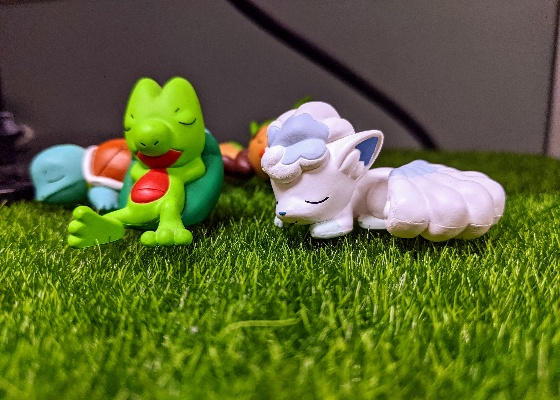
\includegraphics[width=0.7\textwidth]{hw2_sample_images/sample1.jpg}
    \caption{\textbf{sample1.jpg}}
    \label{sample1}
\end{figure}

\subsection{(a)}\label{1_a}
Given an image, \nameref{sample1}.

\subsubsection{(1)}
Perform $1^{\mbox{st}}$ order edge detection and output the edge maps as \nameref{sample1}.

\paragraph{Motivation}
Use non-parametric approaches to conduct edge detection. We could follow the steps of discrete case orthogonal gradient in \textit{Lec 3 page 12 -- 17}.

\paragraph{Approach}
\begin{enumerate}
    \item To-do.
\end{enumerate}

\paragraph{Performance of results}
% Result of problem 1(a): \textbf{1\_result.jpg} \cref{fig1a}.
% \begin{figure}
%     \centering
%     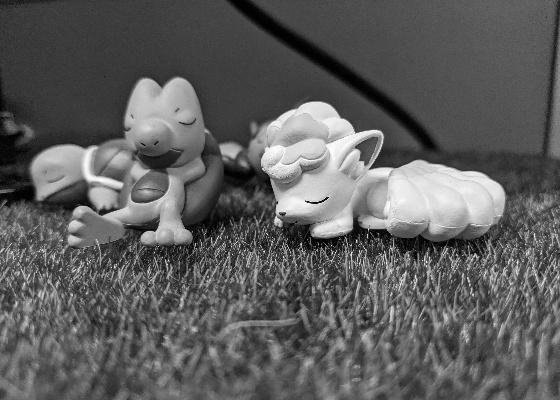
\includegraphics[width=0.7\textwidth]{image/1_result.jpg}
%     \caption{\textbf{1\_result.jpg} Colorful to grayscale}
%     \label{fig1a}
% \end{figure}

\paragraph{Discussion}

\subsection{(b)}

\paragraph{Motivation}

\paragraph{Approach} 

\paragraph{Performance of results}

\paragraph{Discussion}
